\begin{song}{title=\predtitle\centering Zabili \\\large z filmu Balada pro Banditu  \vspace*{-0.3cm}}  %% sem se napíše jméno songu a autor
\begin{centerjustified}
\nejvetsi

\sloka
   ^{C\z }Zabili, ^{F\z }zabili ^{Dmi\z }chlapa z ^{\,\,\,\,F}Koločavy,

   ^{C\z}řekněte ^{F\z}hrobaři, ^{Dmi\z}kde~je ^{\,\,\,\,\,F}pochovaný.


\refren
   ^{C\z }Bylo tu, není tu, havrani ^{F}na plotu,

   ^{C\z }bylo víno v sudě, ^{F\z}teď tam voda bude,

   není, ^{C\z }není tu.


\sloka
   ^{C\z}Špatně ho ^{F\z}zabili, ^{Dmi\z}špatně ^{\,\,\,\,\,F}pochovali,~~

   ^{C\z}vlci ho ^{F\z}pojedli, ^{Dmi}ptáci ^{\,\,\,\,\,F}rozklovali.~~


\refren


\sloka
   ^{C\z}Vítr ho ^{F\z}roznesl ^{Dmi\z}po~dalekém ^{F\z}kraji,

   ^{C\z}havrani ^{F\z}pro~něho ^{Dmi\z}po~poli ^{F}krákají.


\refren


\sloka
   ^{C\z}Kráká ^{\z F}starý havran, ^{Dmi\z}krákat ^{\,\,\,\,\,F}nepřestane,

   ^{C\z}dokud ^{F}v~Koločavě ^{Dmi\z}živý chlap ^{F\:\:}zůstane.


\refren

\end{centerjustified}
\setcounter{Slokočet}{0}
\end{song}


\begin{figure}[h]
\predtitle\centering
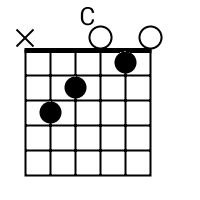
\includegraphics[width=3cm]{../Akordy/c.png}
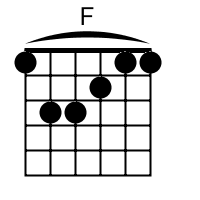
\includegraphics[width=3cm]{../Akordy/f.png}
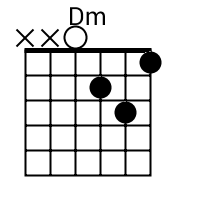
\includegraphics[width=3cm]{../Akordy/dm.png}
\end{figure}
